La gestione delle prenotazioni dei libri è una delle parti innovative introdotte dalla start up: questo servizio mira a sfruttare la flessibilità della community di sharing, basata sull'idea dell'open-source, cercando comunque di offrire un servizio mirato ed attento alle necessità del lettore.

Ogni utente, purchè sia registrato all'interno del servizio di Book-sharing, può prenotare un determinato libro che si trova nello stato "Under reading", ovvero si trova in mano ad un altro utente, il quale lo sta leggendo.

Andiamo ad evidenziare gli attori coinvolti in questa operazione di prenotazione:
\begin{itemize}
	\item \textbf{\underline{Lettore} [L]:} esso rappresenta l'utente, registrato nella community, che possiede il libro oggetto della prenotazione. Indichiamo con:
	\begin{itemize}
		\item \textbf{{\LARGE $r_{L}$}:} raggio d'azione del lettore;
		\item \textbf{{\LARGE $ z_{0} $}:} zona di residenza (espressa come coordinate puntuali).
	\end{itemize}
	\item \textbf{\underline{Prenotanti} [$ P_{i}$ con $i=1,...,N $]:} rappresentano l'insieme degli N utenti, tutti interessati ad uno specifico libro in possesso dell'utente \textbf{L}.
	
	Oltre a questa informazione, ogni utente avrà fornito, al momento della registrazione, i seguenti dati:
	\begin{itemize}
		\item \textbf{{\LARGE $r^{P}_{i}$} con $i=1,...,N $:} raggio d'azione del lettore;
		\item \textbf{{\LARGE $z^{P}_{i}$} con $i=1,...,N $:} zona di residenza.
	\end{itemize}

	L'algoritmo può dunque essere scomposto in due macro-blocchi:
	\begin{itemize}
		\item \textbf{Step 0:} questa fase viene richiamata nel momento in cui il sistema inizia ad analizzare tutti gli utenti che hanno effettuato una prenotazione per un determinato libro che si trova nello stato di \textit{"Under reading"}.
		
		Tutti gli N prenotanti \textit{$ P_{i} $} vengono ordinati in base alla distanza dal lettore \textit{L}, indipendentemente da quello che è l'ordine temporale con cui è stata effettuata la prenotazione: la quantità di cui si terrà (come si può vedere nella figura ~\ref{fig:DistanceAlgorithm}) conto sarà quindi la distanza
		\begin{equation}
			|z^{p}_{i}-z_{0}|
		\end{equation}
		\begin{figure}[h!]
		\centering
		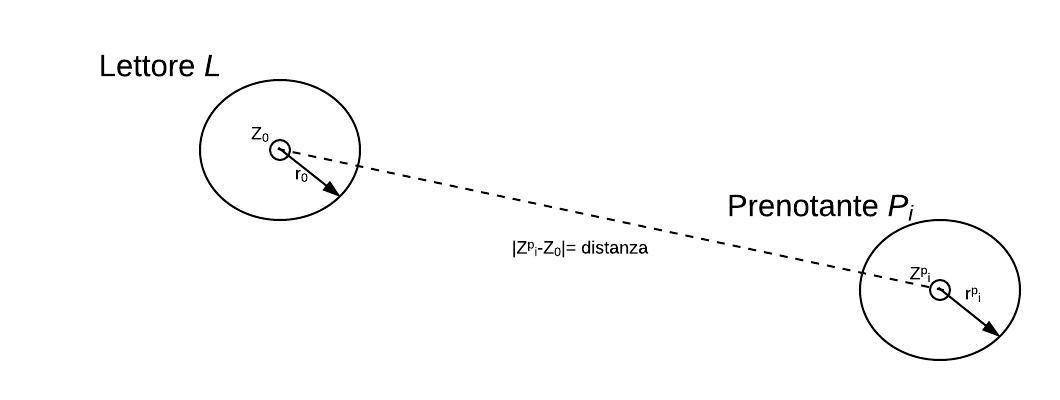
\includegraphics[width=0.8\textwidth]{Immagini/Algoritmo_Explanation}
		\caption{Distanza tra lettore e prenotante i-esimo}
		\label{fig:DistanceAlgorithm}
		\end{figure}
	
		Questo ordinamento corrisponde quindi sostanzialmente a creare una \textit{priority queue} in cui si va ad assegnare una maggiore priorità all'utente la cui zona di residenza è più vicina a quella del lettore in possesso del libro richiesto.
		Nella nostra specifica implementazione, l'ordinamento è stato realizzato tramite l'utilizzo di una SortedMap, con ordinamento \textit{custom} in base al valore (e non secondo la key), ovvero la distanza.
		
		\item \textbf{Step 1:} in questo macro-blocco andiamo effettivamente ad applicare l'algoritmo \textit{smart} per poter soddisfare, nella maniera migliore, le esigenze di ogni utente della community.
		
		
		L'idea di base è che, se utente lettore e utente prenotante hanno possibilità di incontrarsi, ovvero se i loro raggi d'azione si sovrappongono, essi potranno accordarsi direttamente sul luogo dello scambio, rendendo \textit{"safety"} il passaggio del libro: questo scambio avverrà ovviamente in una zona all'interno dell'intersezione dei raggi d'azione, come mostrato in figura ~\ref{fig:Zona_incontro}.
		
		\begin{figure}[h!]
			\centering
			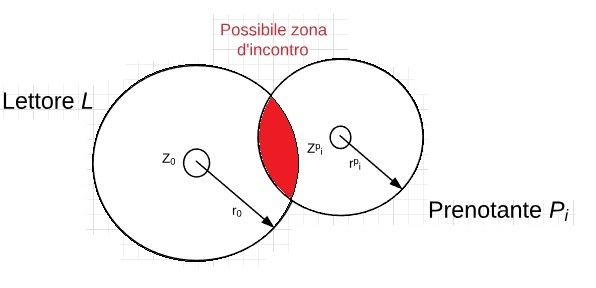
\includegraphics[width=0.6\textwidth]{Immagini/Algorithm_PuntoIncontro.jpg}
			\caption{Zona d'incontro tra lettore e prenotante}
			\label{fig:Zona_incontro}
		\end{figure}
	
		Nel caso in cui invece, i due utenti interessati non abbiano la possibilità di trovare un luogo comune in cui potersi scambiare il libro fisicamente si avrà che, la rete di users appartenenti alla community farà da tramite, per portare il libro \textit{"coast-to-coast"}.
		
		Quindi, tramite un semplice pseudo-codice, possiamo descrivere il nostro algoritmo come
	
		\begin{algorithm}[H]
			\SetAlgoLined
			\KwData{Informazioni dell'utente lettore e di quello prenotante}
			\KwResult{Percorso ottimo dal lettore al prenotante}
			\eIf{Distanza <= 0}{
				Trova un punto d'incontro nell'unione delle delle area;
				
				Notifica gli utenti di dove potersi scambiare direttamente il libro;
			}{
				Crea la rete di utenti che faranno da tramite tra lettore e prenotante;
				
				Ricercare il cammino ottimo (il libro si muoverà \textit{hand-to-hand}) utilizzando \textit{Algorithm 2};
			}
			\caption{Algoritmo di gestione della prenotazione}
		\end{algorithm}
		
		
		Nello specifico il calcolo della distanza avverrà tramite la funzionalità \textit{checkOverlap(Lettore, Prenotante)}, la quale andrà a verificare che:
		
		{\LARGE \begin{equation}
			|z^{p}_{i}-z_{0}|-r_{0}-r_{i}<=0
		\end{equation}}
		
		ovvero che i raggi d'azione si sovrappongano o meno.
		
		Nel caso in cui i due utenti non abbiano possibili punti d'incontro (distanza $>= 0 $), dobbiamo selezionare l'insieme di utenti tramite i quali il libro in questione potrà spostarsi: l'idea base è quindi quella di costruirsi un'area circolare di centro pari alla metà della congiungente del punto $ z_{0} $ (zona di residenza lettore) e $ z^{p}_{i} $ (zona di residenza prenotante).
		
		Verranno poi selezionati tutti gli utenti che si trovano all'interno di questa circoscrizione.
		
		In passi sequenziali, possiamo scrivere:
		
		\begin{algorithm}[H]
			\SetAlgoLined
			\KwData{Zona di residenza e raggio d'azione di tutti gli utenti che si trovano tra lettore e prenotante}
			\KwResult{Elenco di utenti attraverso cui il libro dovrà spostarsi \textit{hand-to-hand}}
			
			
			Il raggio della circoscrizione di utenti coinvolti sarà pari alla distanza
			\[ \bar{Z} = \dfrac{1}{2} |z^{p}_{i}-z_{0}| \]
			\For{ogni utente $ z_{i}^U $ che si trova all'interno della community}{
			\If{$ (Distanza(z_{0},z_{i}^U)) <= \bar{Z} $ oppure $ (Distanza(z_{i}^P,z_{i}^U)) <= \bar{Z} $  }{
				
				Seleziono l'utente $ z_{i}^U $ e lo inserisco nella lista (\textit{HandToHandUsers}) dei possibili utenti che potrebbero partecipare attivamente al prestito;
			}
			}
			Creiamo il collegamento tra gli users della lista \textit{HandToHandUsers} il cui raggio d'azione si sovrappone\;
			\caption{Creazione del percorso tra lettore e prenotante}
		\end{algorithm}
		
		Quindi, alla fine dello step 1, avremo individuato tutti gli utenti i quali possono partecipare attivamente alla realizzazione di un prestito: il risultato ottenuto sarà quindi come quello in figura ~\ref{fig:UsersNet}.
						
		\begin{figure}[h!]
			\centering
			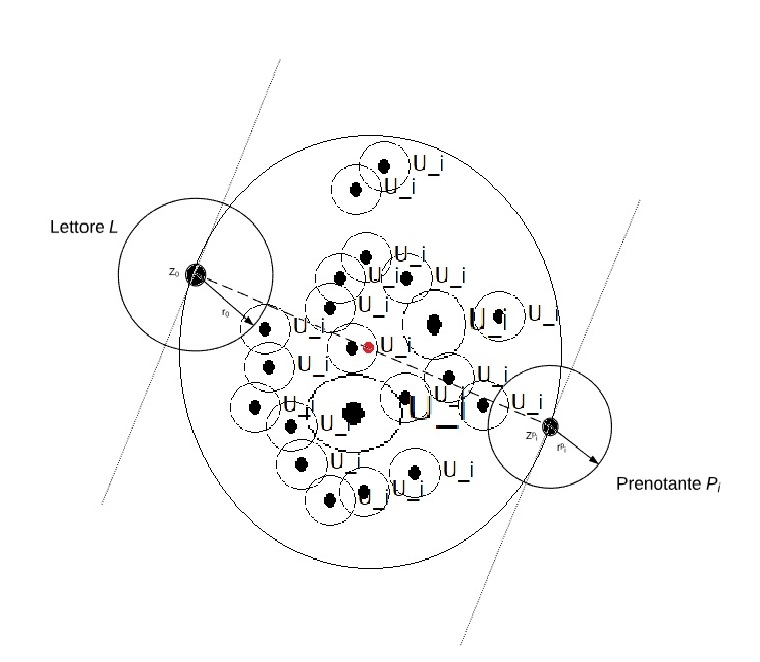
\includegraphics[width=0.8\textwidth]{Immagini/Algorithm_UsersNet}
			\caption{Esempio di rete di utenti che potrebbero essere attivi nel prestito}
			\label{fig:UsersNet}
		\end{figure}
	\end{itemize}
\end{itemize}

Un ulteriore miglioramento che è stato introdotto è rappresentato dal comportamento greedy dell'algoritmo \textit{decisionale}: come è facilmente intuibile, in questo contesto, l'obbiettivo base è quello di andare a minimizzare il numero di km percorsi dal libro, per giungere al lettore prenotante.

Il concetto è quindi quello di minimizzare il numero di utenti che prenderanno parte attivamente al prestito, realizzando un \textit{passamano} tra uno e l'altro.

Un approccio classico per minimizzare il percorso seguito dal libro durante il prestito è quello di andare a scegliere l'utente successivo a cui far arrivare il libro come l'utente la cui distanza è minima tra tutti quelli possibili.

Per rendere però più performante possiamo andare ad applicare un approccio \textit{greedy}, il quale consente di aumentare l'ottimalità dell'algoritmo stesso: nello specifico il concetto seguito nell'implementazione è stato quello di andare ad optare tra due differenti scelte decisionali, ovvero:
\begin{itemize}
	\item \textit{Probabilità $\epsilon$}: andiamo a scegliere l'utente più vicino, tra tutti quelli selezionabili;
	\item \textit{Probabilità $1 - \epsilon$}: tra gli utenti che si possono selezionare, si va a scegliere, con questa probabilità, l'utente con raggio d'azione maggiore
\end{itemize}

Grazie a questa duplice possibile scelta, siamo in grado di rendere l'algoritmo più ottimale, ovvero in grado di trovare, nella maggior parte dei casi, un percorso ottimo; in particolare, minore è il valore di $\epsilon$ che andiamo a scegliere, più \textit{forte} sarà l'algoritmo, ovvero troverà sempre un percorso ma senza garanzia che sia quello ottimale.
Maggiore invece è il valore di $\epsilon$ scelto, più bassa sarà la probabilità che troverà un percorso però, il percorso trovato, sarà uno dei più corti.

\begin{figure}[h!]
	\centering
	\includegraphics[width=0.8\textwidth]{Immagini/Alg_complessità.png}
	\caption{Analisi complessità algoritmo}
	\label{fig:Alg_cmplx}
\end{figure}